\documentclass[10pt,showpacs,preprintnumbers,amsmath,amssymb,nofootinbib,aps,prl,twocolumn,groupedaddress,superscriptaddress,showkeys]{revtex4-1}
\usepackage{graphicx}
\usepackage{dcolumn}
\usepackage{bm}
\usepackage[colorlinks=true,urlcolor=blue,citecolor=blue]{hyperref}
\usepackage{color}
\usepackage{listings}
\usepackage{subfig}
\usepackage{float}
\usepackage{tikz} % Send help 
\usepackage{physics}

\lstset{ %
  basicstyle=\footnotesize,        % the size of the fonts that are used for the code
  breakatwhitespace=false,         % sets if automatic breaks should only happen at whitespace
  breaklines=true,                 % sets automatic line breaking
  captionpos=t,                    % sets the caption-position to bottom
  deletekeywords={...},            % if you want to delete keywords from the given language
  escapeinside={\%*}{*)},          % if you want to add LaTeX within your code
  extendedchars=true,              % lets you use non-ASCII characters; for 8-bits encodings only, does not work with UTF-8
  frame=single,                    % adds a frame around the code
  keepspaces=true,                 % keeps spaces in text, useful for keeping indentation of code (possibly needs columns=flexible)
 % language=Python,                 % the language of the code
  morekeywords={*,...},           % if you want to add more keywords to the set
  numbers=left,                    % where to put the line-numbers; possible values are (none, left, right)
  numbersep=5pt,                   % how far the line-numbers are from the code
  showspaces=false,                % show spaces everywhere adding particular underscores; it overrides 'showstringspaces'
  showstringspaces=false,          % underline spaces within strings only
  showtabs=false,                  % show tabs within strings adding particular underscores
  stepnumber=1,                    % the step between two line-numbers. If it's 1, each line will be numbered
  tabsize=2,                       % sets default tabsize to 2 spaces
}


\begin{document}
\title{FYS3150 Computational Physics - Project 4}
\author{Nicholas Karlsen}


\begin{abstract}
  This is an abstract
\end{abstract}

\maketitle


\section{Introduction}
\section{Theory, Algorithms and Methods}
  \subsection{The Ising Model}
    In its simplest case, a paramagnet is described as a lattice of noninteracting dipole moments, each in a state up or down. Where the energy of the system is proportional to the sum of the spins, up or down of each noninteracting constituent.

    The Ising model is a natural extension to this, by adding local interaction between directly neighboring spins (See fig. \ref{fig:spinsites}), such that the energy of the system is instead proportional to the sum of each spin coupled with its nearest neighbors, which gives a much more accurate description of the system compared to the simple case of an ideal paramagnet.

    Or more precisely, the energy is given by Eqn.~\ref{eqn:ising_energy}, where $s_i \in \{-1, 1\}$ and $J$ is a coupling constant.

    \begin{equation}
      E = -J\sum_{<kl>} s_ks_l
      \label{eqn:ising_energy}
    \end{equation}
    In this summation, the notation $<kl>$ means that for each $k$, we take the sum over each direct neighbor. However, in this project the lattice will be treated as pseudo-continuous where any spin-sites located at an edge, will also interact with the spin-site on the opposing edge, illustrated in Fig.~\ref{fig:ising_periodic bounds}, which strictly speaking constitutes having periodic boundary conditions.

    We also have the magnetization, $\mathcal M$, which is simply the sum of all spins
    \begin{equation*}
      \mathcal M = \sum_i s_i
    \end{equation*}

    \begin{figure}[H]
      \centering
      \begin{tikzpicture}
        [%%%%%%%%%%%%%%%%%%%%%%%%%%%%%%
        dot/.style={circle,draw=black, fill,inner sep=1pt},
        ]%%%%%%%%%%%%%%%%%%%%%%%%%%%%%% 
        \foreach \x in {-1,...,3}{
          \foreach \y in {-1,...,3}{
            % Draw 3x3 dot lattice
            \node[dot] at (\x,\y){};
            \node[dot] at (\x,\y){};
          }
        }
        \draw[thick, dashed] (1 + .1 , 1) -- (1 + 0.9, 1);
        \draw[thick, dashed] (1 - .1 , 1) -- (1 - 0.9, 1);
        \draw[thick, dashed] (1, 1 + .1) -- (1, 1 + 0.9);
        \draw[thick, dashed] (1, 1 - .1) -- (1, 1 - 0.9);
        % Text 
        \draw (1+.25, 1+.2) node{$s_{k}$};
      \end{tikzpicture}
      \caption{Section of a 2D lattice, where each spin-site is represented by a dot. In the Ising model, spin-site $k$ will only interact with its directly neighbouring spin-sites, connected by dotted lines in this diagram\label{fig:spinsites}}
    \end{figure}
      \begin{figure}[H]
      \centering
      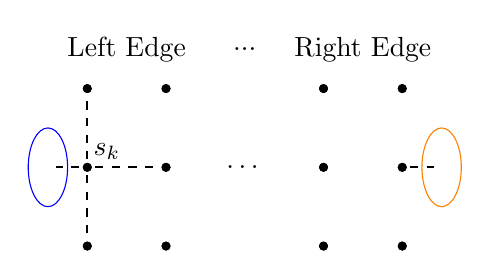
\begin{tikzpicture}
        [%%%%%%%%%%%%%%%%%%%%%%%%%%%%%%
        dot/.style={circle,draw=black, fill,inner sep=1pt},
        ]%%%%%%%%%%%%%%%%%%%%%%%%%%%%%% 
        \foreach \x in {2,...,1}{
          \foreach \y in {-1,...,1}{
            % Draw 3x3 dot lattice
            % LEFT LATTICE
            \node[dot] at (-\x,\y){};
            \node[dot] at (-\x,\y){};
            % RIGHT LATTICE
            \node[dot] at (\x,\y){};
            \node[dot] at (\x,\y){};
          }  
        }    
        % Lines
        \draw[thick, dashed] (-2, 0 + .1) -- (-2, 1 - .1);
        \draw[thick, dashed] (-2, 0 - .1) -- (-2, -1 + .1 );
        \draw[thick, dashed] (-2 + .1, 0) -- (-1 - .1, 0);

        \draw[color=blue] (-2.5,0) ellipse (0.25cm and .5cm);
        % Portal lines
        \draw[thick, dashed] (-2 - .1, 0) -- (-2.5 + .1, 0);
        \draw[thick, dashed] (2 + .1, 0) -- (2.5 - .1, 0);
        \draw[color=orange] (2.5,0) ellipse (0.25cm and .5cm);
        % Text
        \draw (0, 0) node{$\dots$};
        \draw (-1.5, 1.5) node{Left Edge};
        \draw (1.5, 1.5) node{Right Edge};
        \draw (0, 1.5) node{...};
        \draw (-2+.25, 0+.2) node{$s_{k}$};
      \end{tikzpicture}
      \caption{Spin-site $k$, located at the left edge of the lattice interacting with its direct neighbors, as well as the spin site on the opposite edge of the lattice
      \label{fig:ising_periodic bounds}}
    \end{figure}

    \subsubsection{Boltzmann Statistics}
      From Eqn.~\ref{eqn:ising_energy} we can derive many thermodynamic quantities using Boltzmann statistics, where we have the probability of the system being in some specific macro-state\footnote{Macroscopic states being characterized by their energy, meaning i could just as well have written "... the probability of the system having some speciffic energy"}
      \begin{equation}
        \mathcal P(E_s) = \frac{1}{Z} e^{-\beta E_s}
      \end{equation}
      With $\beta \equiv \frac{1}{k_B T}$, the thermodynamic beta and $Z$, the partition function, acting as a normalization factor given by\footnote{Strictly speaking, this is the partition function for a system with discrete macro-states. In the continuous case, simply replace sums with integrals.}

      \begin{equation}
        Z = \sum_s e^{-\beta E_s}
      \end{equation}
      From this, the expectation value of some quantity $X$, with a set of known macrostates $X_s$ can be computed by

      \begin{equation}
        \left<X\right> = \sum_s X_s \mathcal P(E_s) = \frac{1}{Z} \sum_s X_s e^{-\beta E_s} 
      \end{equation}
      Using this, we can compute the specific heat capacity, $C_V$ by computing the expectation values of $E, E^2$ \cite{statmek_lecnotes}, related by the following expression

      \begin{equation}
        C_V = \frac{\left<E^2\right> - \left<E\right>^2}{k_B T^2}
      \end{equation}
      Where $\left<X^2\right> - \left<X\right>^2$ is recognized as the square of the standard deviation in the normal distribution, $\sigma_X^2$.

      In a similar fashion, the magnetic susceptibility, $\chi$, is calculated from $\sigma_\mathcal M ^2$ \cite{statmek_lecnotes}

      \begin{equation}
        \chi = \frac{\sigma^2_\mathcal M}{k_B T}
      \end{equation}

      For more details on the Ising model, or Boltzmann statistics refer to \textcite[Chapters~6, 8.2]{schroeder}, \textcite{statmek_lecnotes}, or similar introductory texts on the topic.

  \subsubsection{Analytic solution of 2x2 Lattice}
    Consider now a 2x2 lattice, each with spin $\pm 1$.
    The energy of the system for a particular micro-state is given by Eqn.~\ref{eqn:ising_energy}.

     \begin{figure}[H]
      \centering
      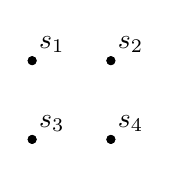
\begin{tikzpicture}
        [%%%%%%%%%%%%%%%%%%%%%%%%%%%%%%
        dot/.style={circle,draw=black, fill,inner sep=1pt},
        ]%%%%%%%%%%%%%%%%%%%%%%%%%%%%%% 
        \foreach \x in {0,...,1}{
          \foreach \y in {0,...,1}{
            % Draw 3x3 dot lattice
            \node[dot] at (\x,\y){};
            \node[dot] at (\x,\y){};
          }
        }
        \draw (0+.25, 1+.2) node{$s_{1}$};
        \draw (1+.25, 1+.2) node{$s_{2}$};
        \draw (0+.25, 0+.2) node{$s_{3}$};
        \draw (1+.25, 0+.2) node{$s_{4}$};

      \end{tikzpicture}
      \caption{A $2\times2$ lattice of spin-sites}
    \end{figure}

  \subsection{The Metropolis Algorithm}

\section{Results and Discussions}

\section{Conclusions}

\bibliography{../bibliography.bib}


\end{document}  